\documentclass{../zkdl-presentation-template}

\title[Криптографія]{\textbf{Практичне №4.ЛРЗ. Блокові Шифри: Схема Фейстеля, режими БШ}}

\date{23.09.2025}


\begin{document}
    \frame{
        \titlepage
    }
  
    \begin{frame}{Plan}
        \tableofcontents
    \end{frame}

\section{ЛРЗ} % Note all sections and subsections are automatically placed in your table of contents

%------------------------------------------------
\begin{frame}
    \frametitle{Визначення. Повторення}
\begin{block}{}
    \begin{itemize}
        \item Виходи ЛРЗ формують деяку цикличні послідовність
        \item Для початку роботи задається початковий стан (не нульовий!!!)
    \end{itemize}
\end{block}
\begin{figure}
    \centering
    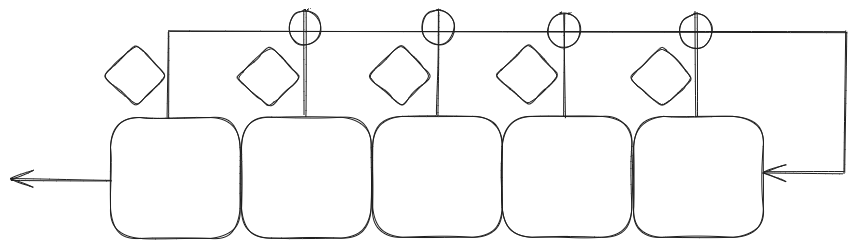
\includegraphics[width=0.65\linewidth]{3-crypto-practice/images/LRZ.png}
\end{figure}
\end{frame}
%------------------------------------------------
\begin{frame}{Задача}
    \begin{block}{}
        За відрізком лінійної рекурентної послідовності над $\mathtt{GF}(2)$ --- $(s_i...s_{i+7})=(00010110)$ побудувати регістр зсуву з лінійним зворотним зв'язком довжини $4$, що її породжує.
    \end{block}
    \begin{figure}
        \centering
        
\includegraphics[width=1\linewidth]{2-crypto-sym/images/cells.png}
    \end{figure}
\end{frame}
%------------------------------------------------
\section{Схема Фейстеля}
%------------------------------------------------
\begin{frame}{Загальна схема}
\begin{columns}[c] % [c] вирівнювання по центру вертикалі
        \column{0.5\textwidth}
    \begin{figure}
        \centering
        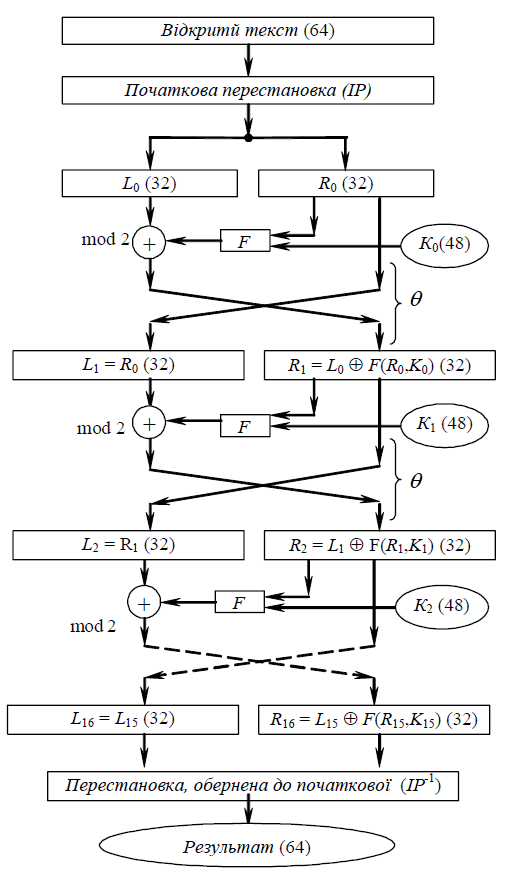
\includegraphics[width=0.84\linewidth]{4-crypto-practice/images/Feistel_scheme.png}
    \end{figure}
        \column{0.5\textwidth}
        \begin{block}{}
            \begin{itemize}
                \item Доведіть, що один раунд схеми Фейстеля (без фінальної перестановки) є інволютивним шифром;
                \item Чому раундове перетворення $f(L,R)$ має бути бієкцією
                \item Довести, що алгоритм розшифрування відрізняється від алгоритму шифрування лише зворотним порядком подачі циклових ключів.
            \end{itemize}
        \end{block}
    \end{columns}
\end{frame}
%------------------------------------------------
\begin{frame}{Задача}
    \begin{block}{}
        Сімейство блокових шифрів MISTY побудовано на основі $L$-схеми, в якій раунд має вид $F_k(x,y)=(y,y\bigoplus f_k(x))$. Накресліть схеми шифрування та розшифрування (один раунд). Чи буде ця схема інволютивною при зворотній подачі ключів? Чи $f$ -- обов'язково бієкція?
    \end{block}
    \begin{figure}
        \centering
        
\includegraphics[width=1\linewidth]{2-crypto-sym/images/cells.png}
    \end{figure}
\end{frame}
%------------------------------------------------
\section{Режими блокових шифрів}
%------------------------------------------------
\begin{frame}{ECB}
\begin{figure}
    \centering
    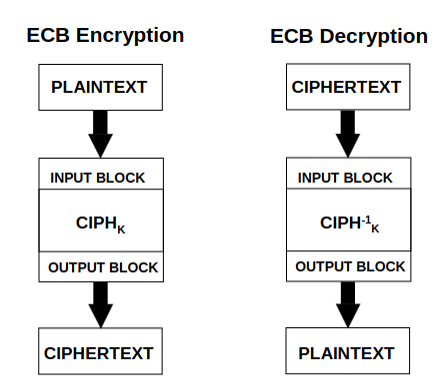
\includegraphics[width=0.5\linewidth]{4-crypto-practice/images/ECB.png}
\end{figure}
    \begin{figure}
        \centering
        
\includegraphics[width=1\linewidth]{2-crypto-sym/images/cells_small.png}
    \end{figure}
\end{frame}
%------------------------------------------------
\begin{frame}{CBC}
\begin{figure}
    \centering
    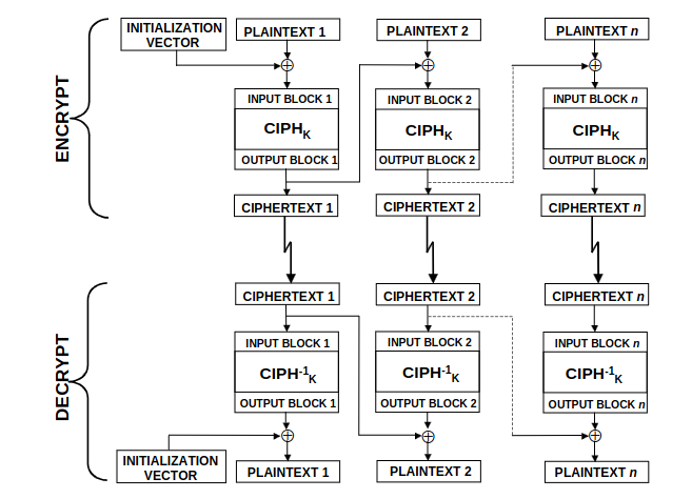
\includegraphics[width=0.65\linewidth]{4-crypto-practice/images/CBC.png}
\end{figure}
\vspace{-3mm}
    \begin{figure}
        \centering
        
\includegraphics[width=1\linewidth]{2-crypto-sym/images/cells_small.png}
    \end{figure}
\end{frame}
%------------------------------------------------
\begin{frame}{CFB}
\begin{figure}
    \centering
    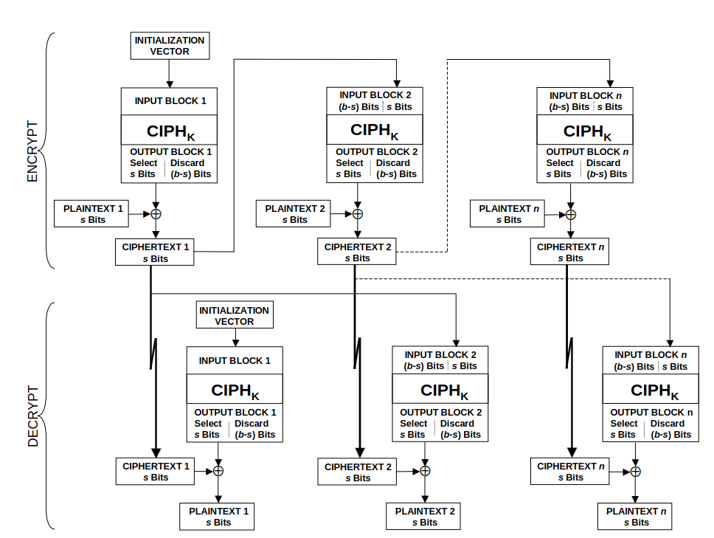
\includegraphics[width=0.65\linewidth]{4-crypto-practice/images/CFB.png}
\end{figure}
\vspace{-3mm}
    \begin{figure}
        \centering
        
\includegraphics[width=1\linewidth]{2-crypto-sym/images/cells_small.png}
    \end{figure}
\end{frame}
%------------------------------------------------
\begin{frame}{OFB}
\begin{figure}
    \centering
    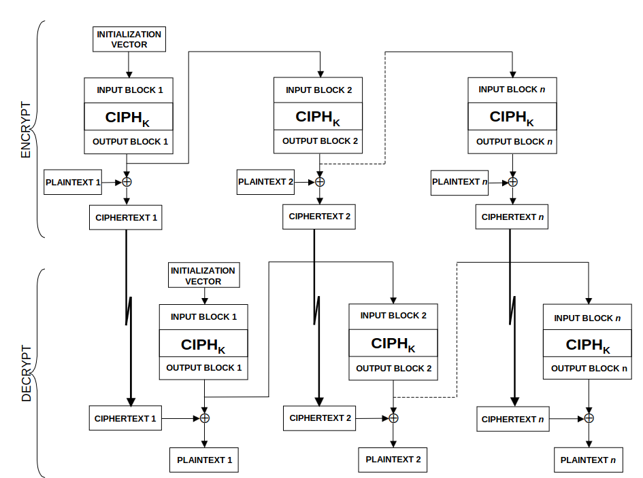
\includegraphics[width=0.65\linewidth]{4-crypto-practice/images/OFB.png}
\end{figure}
\vspace{-3mm}
    \begin{figure}
        \centering
        
\includegraphics[width=1\linewidth]{2-crypto-sym/images/cells_small.png}
    \end{figure}
\end{frame}
%------------------------------------------------
\begin{frame}{CTR}
\begin{figure}
    \centering
    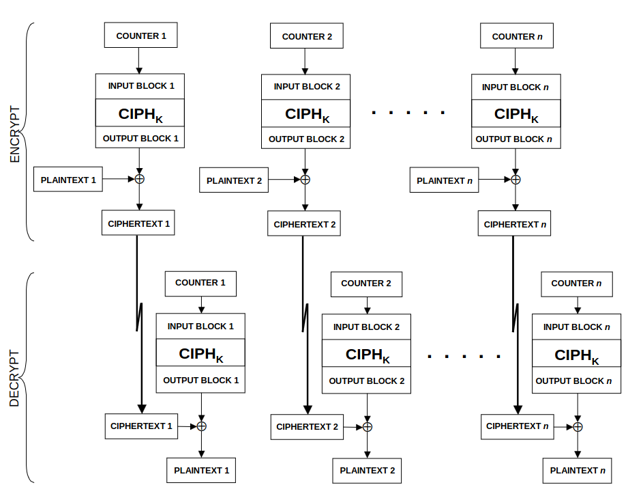
\includegraphics[width=0.65\linewidth]{4-crypto-practice/images/CTR.png}
\end{figure}
\vspace{-3mm}
    \begin{figure}
        \centering
        
\includegraphics[width=1\linewidth]{2-crypto-sym/images/cells_small.png}
    \end{figure}
\end{frame}
%------------------------------------------------
\section{Відстань однозначності}
%------------------------------------------------
\begin{frame}{Задача}
    \begin{figure}
        \centering
        
\includegraphics[width=1\linewidth]{2-crypto-sym/images/cells.png}
    \end{figure}
\end{frame}
%------------------------------------------------
\section{Шифр AES}
%-----------------------------------------------
    \begin{frame}{AES --- сучасний блоковий шифр}
            \begin{figure}
                \centering
                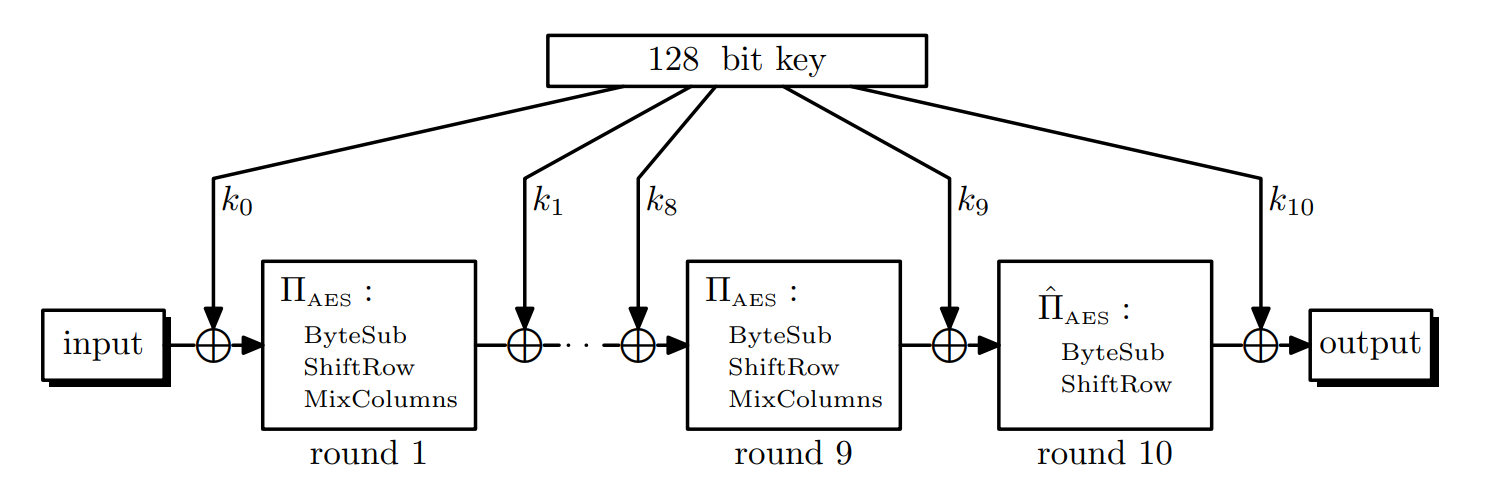
\includegraphics[width=0.9\linewidth]{4-crypto-practice/images/AES_scheme.png}
            \end{figure}
          \begin{definition}
            \textbf{AES} (ориг.RIJNDAEL) --- стандартизований ітеративний блоковий шифр, прийнятий NIST у 2002 році. Кількість раундів цього шифру залежить від довжини ключа, а раундова функція складається з трьох алгоритмів, що працюють з матрицями фіксованого розміру $4\times4$ (байт): \texttt{SybBytes, ShiftRows, MixColumns}.
          \end{definition}
          \vspace{-3.5mm}
          \centering Візуальну роботу AES можна подивитися за  \textcolor{blue}{\href{https://legacy.cryptool.org/en/cto/aes-animation}{цим посиланням}}.          
    \end{frame}

    \begin{frame}{Раундова функція AES}
        \begin{figure}
            \centering
            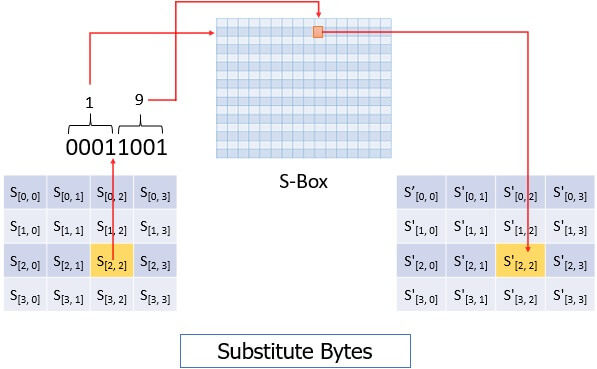
\includegraphics[width=0.65\linewidth]{4-crypto-practice/images/Substitute-Bytes.jpg}
        \end{figure}
        \begin{figure}
            \centering
            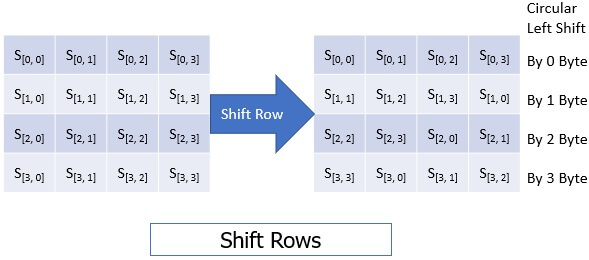
\includegraphics[width=0.65\linewidth]{4-crypto-practice/images/Shift-Rows.jpg}
        \end{figure}
    \end{frame}

    \begin{frame}{Раундова функція AES}
        \begin{figure}
            \centering
            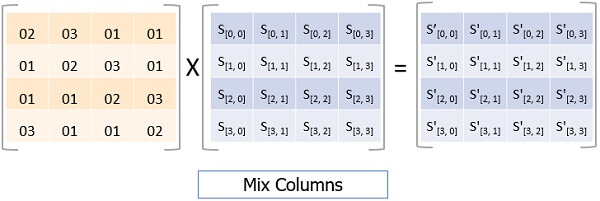
\includegraphics[width=0.8\linewidth]{4-crypto-practice/images/Mix-Columns.jpg}
        \end{figure}
        \begin{figure}
            \centering
            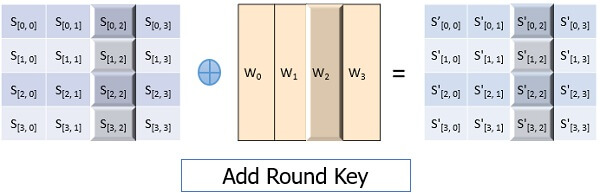
\includegraphics[width=0.8\linewidth]{4-crypto-practice/images/Add-Round-Key.jpg}
        \end{figure}
    \end{frame}

    \begin{frame}[plain, standout]
    \begin{figure}
        \centering
        
\includegraphics[width=0.9\linewidth]{Cryptocats.jpg}
        \label{fig:placeholder}
    \end{figure}
    \centering
    \LARGE
    \textbf{Питання?} \\

    \vspace{0.2cm} \Huge \ding{170} \large \\

  \end{frame}
\end{document}